\documentclass{article}
\usepackage[utf8]{inputenc}

\title{Week 8 Lecture 2}
\author{Jared Brannan }

\usepackage{natbib}
\usepackage{graphicx}
\graphicspath{ {./figures/} }
\usepackage{mathtools}
\usepackage{amsthm}
\usepackage{amsmath}
\usepackage{amssymb}
\usepackage{xcolor}
\usepackage{bbm}
\usepackage{bm}
\usepackage{physics}

% indent first line
\usepackage{indentfirst}
% one inch margins
\usepackage[margin=1.0in]{geometry}

\theoremstyle{definition}

\newcommand{\upRiemannint}[2]{
\overline{\int_{#1}^{#2}}
}
\newcommand{\loRiemannint}[2]{
\underline{\int_{#1}^{#2}}
}

\newtheorem{definition}{Definition}
\newtheorem{asside}{Asside}
\newtheorem{conjecture}{Conjecture}
\newtheorem{example}{Example}
\newtheorem{theorem}{Theorem}
\newtheorem{lemma}{Lemma}
\newtheorem{puzzle}{Puzzle}
\newtheorem{corollary}{Corollary}
\newtheorem{proposition}{Proposition}


\begin{document}
\maketitle

\section{Administrative drivel}
\begin{itemize}
	\item The 2nd draft of the paper is \textbf{not} due today -- to be anounced.
\end{itemize}

\section{Anatomy and Physiology}

\subsection{Cardiovascular system continued...}
\subsubsection{Cardiovascular disease: blood vessels}
\begin{itemize}
	\item Most CVD (cardiovascular disease) is caused by blockages in the vessels
	\item \textbf{Atherosclerosis} is the hardening of the blood vessels
		\begin{itemize}
			\item Colesterol accumulates in one spot (in the wall) forming a plaque
			\item Blood can clot at the plaque forming a \textbf{Thrombus} 
			\item Obstructed artery increases blood pressure
			\item Thrombus can break free to lodge in and block a smaller vessel == \textbf{embolus} 
			\item An \textbf{embolism} is a blocked vessel
			\item if the thrombus gets loose, it can move to a vessel with a smaller diameter, blocking the vessel, which can cause a stroke or heart attack
			\item they form more in the legs in older people
		\end{itemize}
	\item \textbf{Myocardial infarction}  (heart attack)
		\begin{itemize}
			\item Death of part of the heart beause its own blood suply is blocked
				\begin{itemize}
					\item the muscle has to switch to anarobic (eek)
				\end{itemize}
			\item typically from a thrombus in the coronary arteries
			\item temporary loss of $O_2$ makes heart act like a cramped muscle $\to$ pain $\equiv$ \textbf{angina} 
		\end{itemize}
	\item Bipass surgery is one of the ways to deal with one of these obstructions
		\begin{itemize}
			\item A vessel is inserted to bypass the blocked area
			\item this is very effective, but usually only viable for about 15 years.
			\item more common in men
		\end{itemize}
	\item \textbf{Aneurysm}  (weakened vessel -- \underline{artery} or vein)
		\begin{itemize}
			\item Weak spot in artery ballons under pressure
			\item weak spot can burst,  causing internal bleeding
			\item for arteries outside the brain, the weakened artery can be sheethed
		\end{itemize}
	\item \textbf{Stroke:} embolism or aneurysm in the brain
		\begin{itemize}
			\item Symptons include loss of motor function, sensation, speech, or vision
			\item typically on one side of the body
			\item symptoms can be reversed if get to the hospital within minutes
		\end{itemize}
	\item \textbf{Hypertension:} high blood pressure
		\begin{itemize}
			\item Systolic BP > 140 mmHG
			\item Diastolic BP > 90 mmHG
			\item causes: diet, genetics
			\item key risk: capillaries leak or burst, leading to stroke
		\end{itemize}
\end{itemize}

\subsection{Respiratory system}
\begin{itemize}
	\item Functions:
		\begin{itemize}
			\item Acquire $O_2$
			\item Expel $CO_2$
			\item Maintain blood pH -- by regulating $CO_2$ (spits into carbonic acid $HCO_3$ and a hydrogen ion, the latter elevates the pH)
			\item pH at tissue is slightly higher allowing oxygen to more easily disolve into the blood
			\item Produce sound
		\end{itemize}
	\begin{center}
		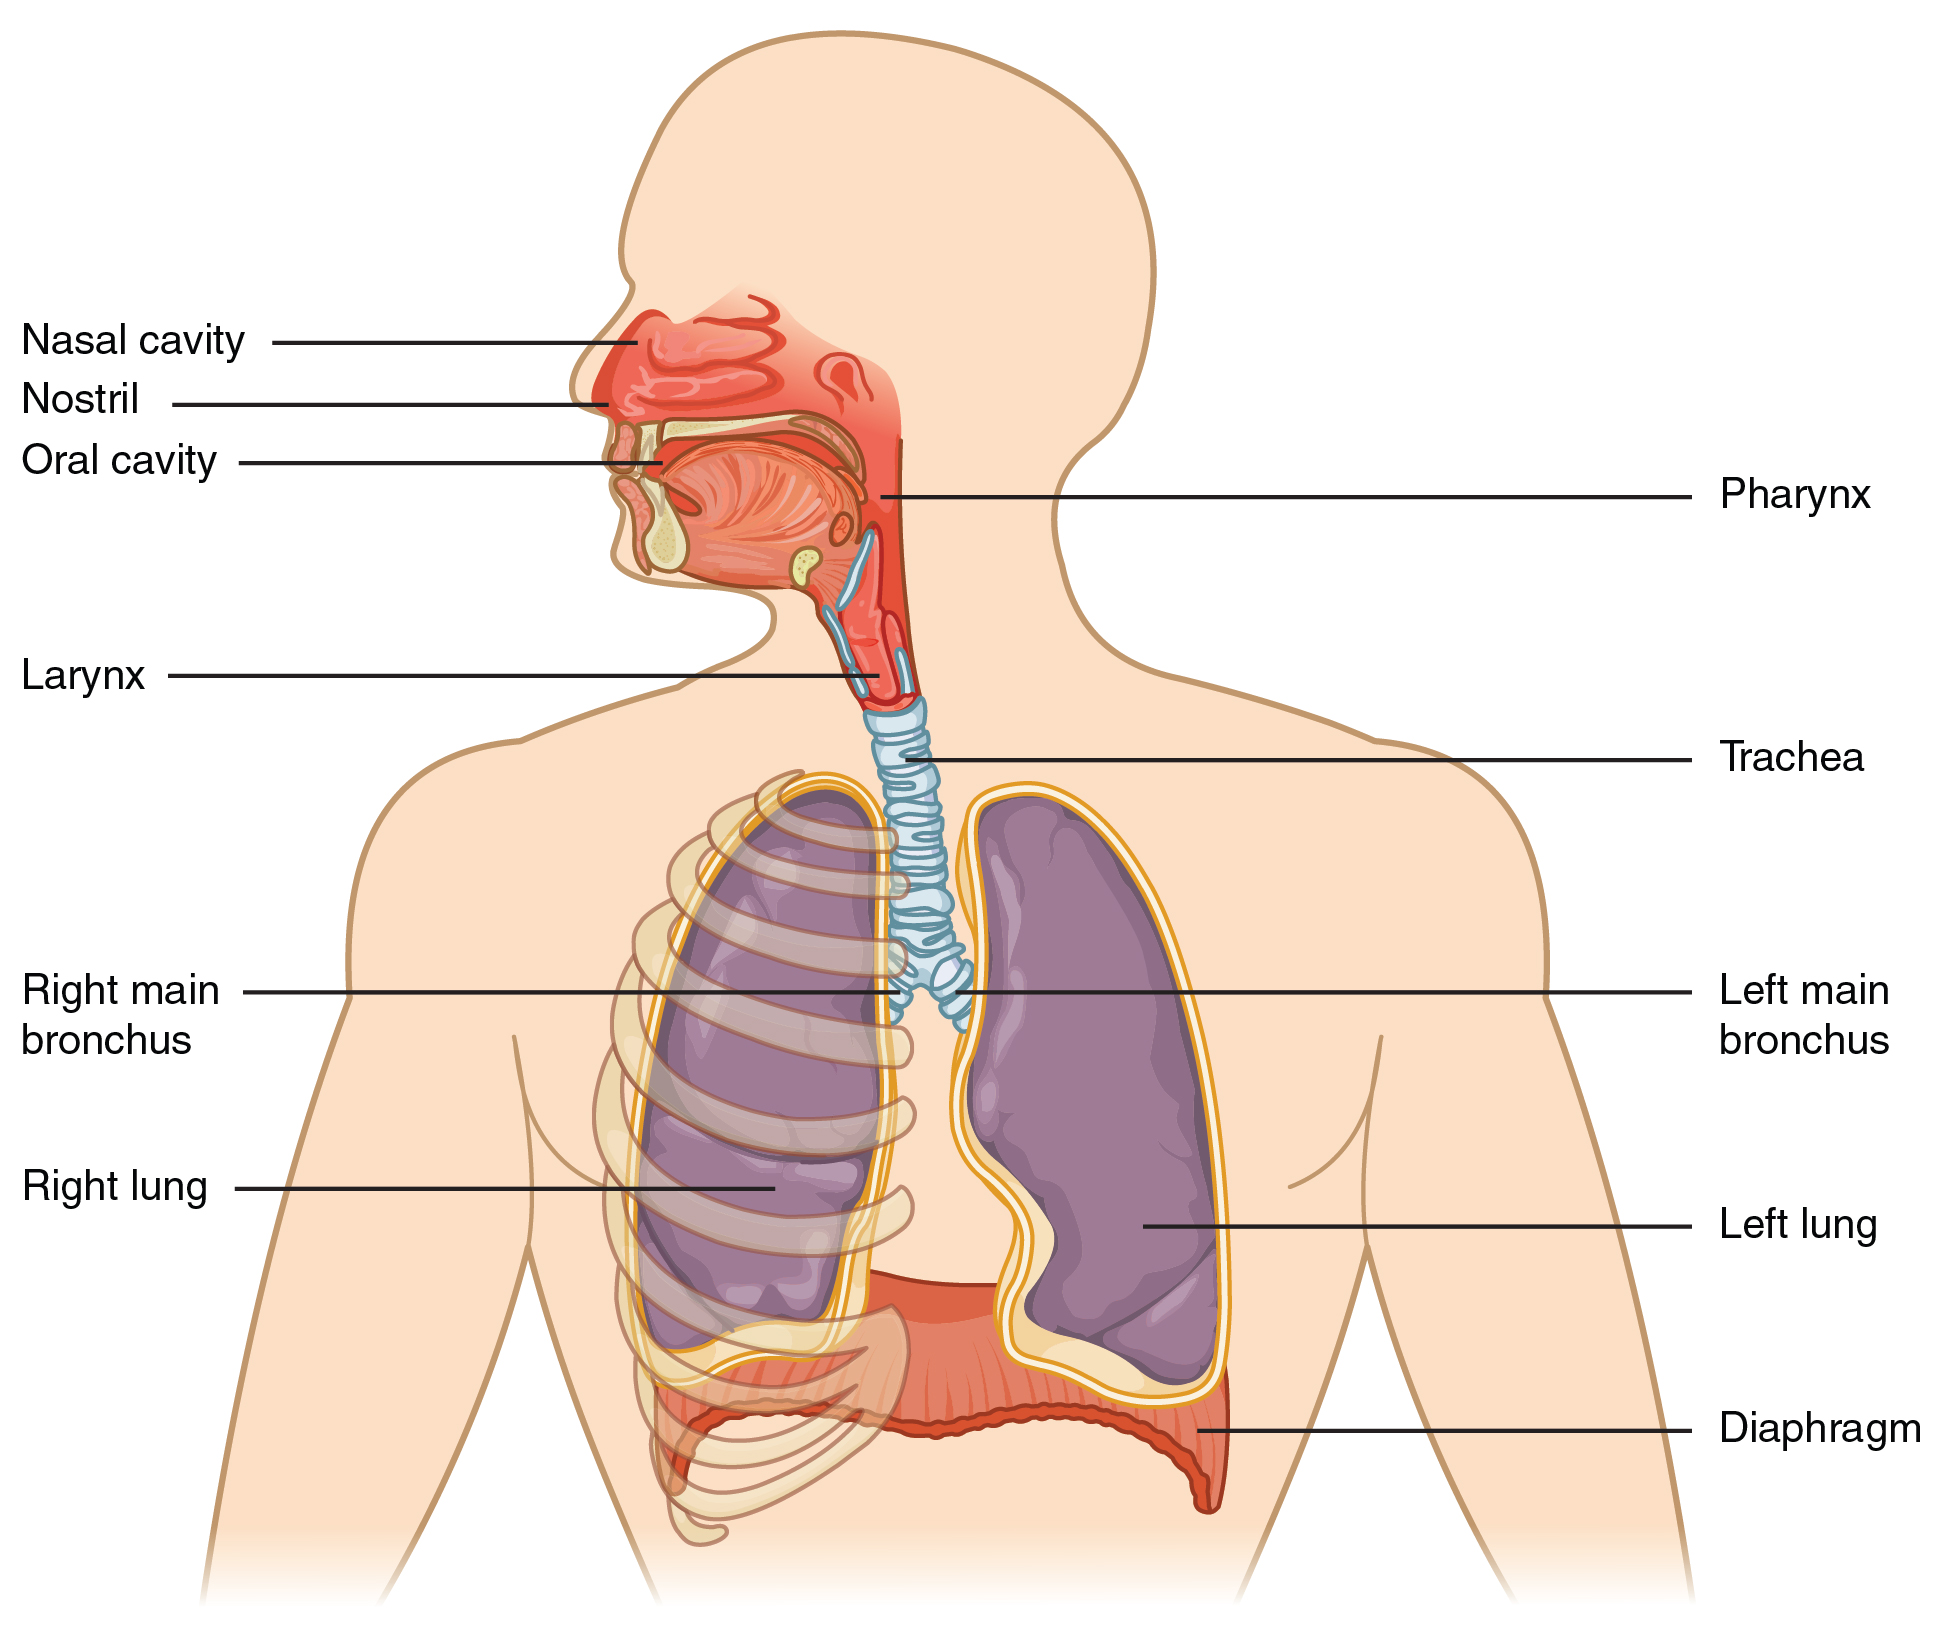
\includegraphics[width=30em]{Respiratory_Organs.jpg}
	\end{center}
	\item Upper resperiatory tract:
		\begin{itemize}
			\item Nose, mouth, and pharynx
				\begin{itemize}
					\item nasal cavity, nostril, oral cavity, pharynx, larynx
					\item brings in air
					\item warms, moistens, and filters air
					\item air in the lungs it 100\% humidity
				\end{itemize}
			\item When breathing in, the nasal bones cool, warming the air, and vice versa on the way out (likewise, condensation in the nose humidifies the air, and recondenses in the nasal cavity on the way out)
			\item Trachea
				\begin{itemize}
					\item Move air from upper tract to lungs
					\item carilage holds tracheo open
					\item smooth muscle between that can change the size of the trachea
				\end{itemize}
			\item Bronchial tree
				\begin{itemize}
					\item bronchi, to the bronchioles,, then at the end of the broonchiloi are Alveoli
				\end{itemize}
			\item Alveoli are where the gass exchange occurs (looks like a little grape)
				\begin{itemize}
					\item large surfaace area
				\end{itemize}
		\end{itemize}
\end{itemize}


\end{document}
